

\tikzset{every picture/.style={line width=0.75pt}} %set default line width to 0.75pt        

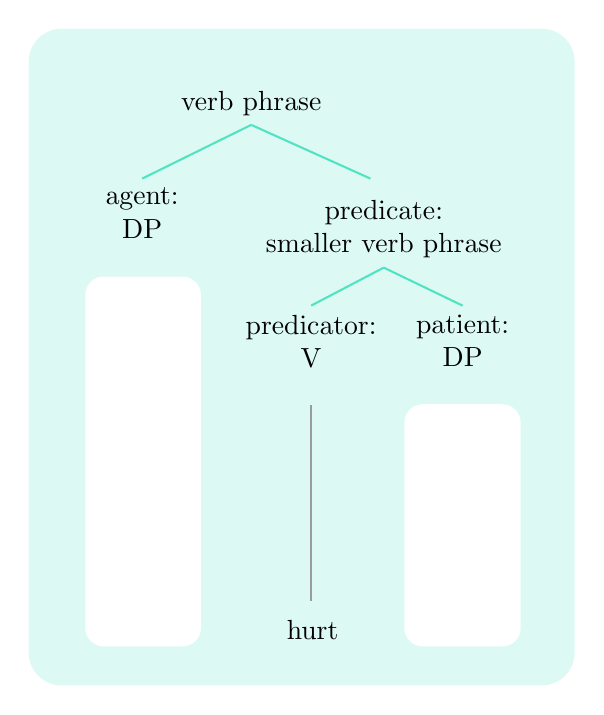
\begin{tikzpicture}[x=0.75pt,y=0.75pt,yscale=-1,xscale=1]
%uncomment if require: \path (0,359); %set diagram left start at 0, and has height of 359

%Rounded Rect [id:dp9005470977487176] 
\draw  [draw opacity=0][fill={rgb, 255:red, 80; green, 227; blue, 194 }  ,fill opacity=0.2 ] (264,45.22) .. controls (264,36.48) and (271.08,29.4) .. (279.82,29.4) -- (511.18,29.4) .. controls (519.92,29.4) and (527,36.48) .. (527,45.22) -- (527,329.99) .. controls (527,338.73) and (519.92,345.81) .. (511.18,345.81) -- (279.82,345.81) .. controls (271.08,345.81) and (264,338.73) .. (264,329.99) -- cycle ;
%Straight Lines [id:da3555404365615693] 
\draw [color={rgb, 255:red, 155; green, 155; blue, 155 }  ,draw opacity=1 ]   (400.05,210.81) -- (400.05,305) ;
%Straight Lines [id:da5116688308518689] 
\draw [color={rgb, 255:red, 80; green, 227; blue, 194 }  ,draw opacity=1 ]   (473.05,162.83) -- (435.05,144.5) ;
%Straight Lines [id:da7532901881200198] 
\draw [color={rgb, 255:red, 80; green, 227; blue, 194 }  ,draw opacity=1 ]   (435.05,144.5) -- (400.05,162.83) ;
%Straight Lines [id:da3708728686228633] 
\draw [color={rgb, 255:red, 80; green, 227; blue, 194 }  ,draw opacity=1 ]   (428.65,101.63) -- (371.2,75.73) ;
%Straight Lines [id:da18650265857430104] 
\draw [color={rgb, 255:red, 80; green, 227; blue, 194 }  ,draw opacity=1 ]   (371.2,75.73) -- (318.65,101.63) ;
%Rounded Rect [id:dp9951745940140804] 
\draw  [draw opacity=0][fill={rgb, 255:red, 255; green, 255; blue, 255 }  ,fill opacity=1 ] (445,219.16) .. controls (445,214.29) and (448.95,210.33) .. (453.83,210.33) -- (492.17,210.33) .. controls (497.05,210.33) and (501,214.29) .. (501,219.16) -- (501,318.17) .. controls (501,323.05) and (497.05,327) .. (492.17,327) -- (453.83,327) .. controls (448.95,327) and (445,323.05) .. (445,318.17) -- cycle ;
%Rounded Rect [id:dp4970986462373306] 
\draw  [draw opacity=0][fill={rgb, 255:red, 255; green, 255; blue, 255 }  ,fill opacity=1 ] (291.24,157.76) .. controls (291.24,152.82) and (295.25,148.81) .. (300.19,148.81) -- (338.05,148.81) .. controls (342.99,148.81) and (347,152.82) .. (347,157.76) -- (347,318.05) .. controls (347,322.99) and (342.99,327) .. (338.05,327) -- (300.19,327) .. controls (295.25,327) and (291.24,322.99) .. (291.24,318.05) -- cycle ;

% Text Node
\draw (400.76,325) node [anchor=south] [inner sep=0.75pt]   [align=left] {hurt};
% Text Node
\draw (435.05,141.5) node [anchor=south] [inner sep=0.75pt]   [align=left] {\begin{minipage}[lt]{89.53pt}\setlength\topsep{0pt}
\begin{center}
predicate:\\smaller verb phrase
\end{center}

\end{minipage}};
% Text Node
\draw (371.2,72.73) node [anchor=south] [inner sep=0.75pt]   [align=left] {verb phrase};
% Text Node
\draw (318.65,104.63) node [anchor=north] [inner sep=0.75pt]   [align=left] {\begin{minipage}[lt]{29.61pt}\setlength\topsep{0pt}
\begin{center}
agent:\\DP
\end{center}

\end{minipage}};
% Text Node
\draw (400.05,165.83) node [anchor=north] [inner sep=0.75pt]   [align=left] {\begin{minipage}[lt]{50.89pt}\setlength\topsep{0pt}
\begin{center}
predicator:\\V
\end{center}

\end{minipage}};
% Text Node
\draw (473.05,165.83) node [anchor=north] [inner sep=0.75pt]   [align=left] {\begin{minipage}[lt]{36.95pt}\setlength\topsep{0pt}
\begin{center}
patient:\\DP
\end{center}

\end{minipage}};


\end{tikzpicture}
